% !TEX root = ../main.tex
\chapter{Үр дүн}\label{ch:results}\label{ch:perf}

\section{Тестийн үр дүн}
100 автомат тест хоёр орчинд хоёуланд нь амжилттай (100/100) болсон. Lockstep-ийн тестийг 30 удаа давтаж,
нэг цөм дээр ажиллуулахад ч алдаа гараагүй. Тест бүрийн оролт, хүлээгдсэн ба бодит утгыг
\code{tests/results/test-results.md}-д өгөв.

\begin{figure}[H]
\centering
\IfFileExists{images/test-run-mac.png}{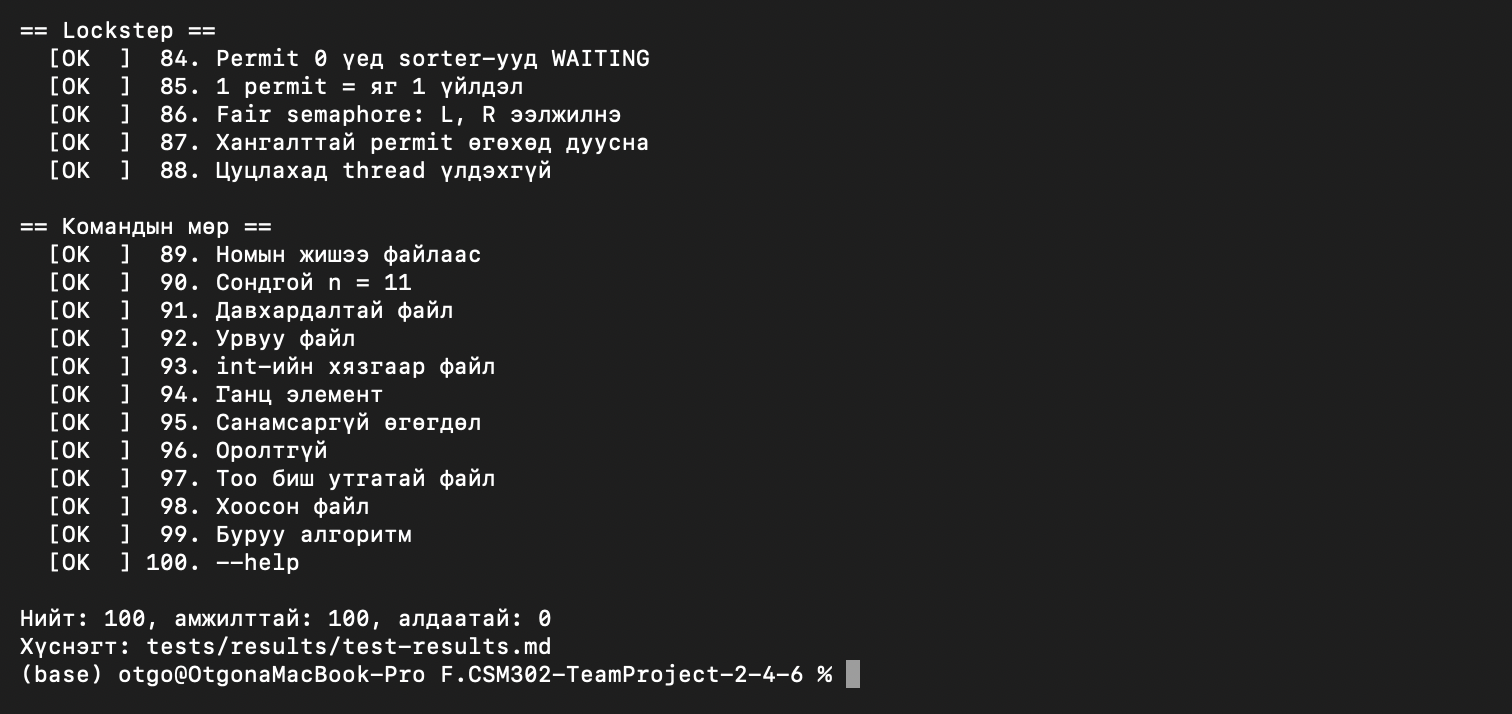
\includegraphics[width=0.7\linewidth]{images/test-run-mac.png}}{%
\fbox{\parbox[c][3cm][c]{0.7\linewidth}{\centering\color{cparent}Энд зураг оруулна: \texttt{report/images/test-run-mac.png}}}}
\caption{\code{./test.sh}-ийн гаралт}\label{fig:testrun}
\end{figure}

\section{Хугацааны хэмжилтийн үр дүн}
Хүснэгт~\ref{tab:bench}-т $n$-ийн хамгийн том утгууд дээрх үр дүнг, Зураг~\ref{fig:bench-speedup}-т зэрэгцээний
хурдсалтыг $n$-ээс хамааруулан харуулав. Бүрэн үр дүн \code{tests/results/benchmark.md}-д бий.

\begin{table}[H]
\centering
\caption{Хугацаа (ms, медиан). Хаалтанд 3 thread-ийн JVM хоорондын муж}\label{tab:bench}
\resizebox{\linewidth}{!}{%
\begin{tabular}{@{}lrrrrrrr@{}}
\toprule
Алгоритм & $n$ & 1 thread & 1 thr., хувааж & 3 thread & Нэгтгэх үе & Нийт & Зэрэгц. \\
\midrule
insertion & 20 000 & 180.1 & 90.6 & 50.6 (48.3--54.3) & 0.7 & 3.56 & 1.79 \\
bubble & 20 000 & 466.1 & 198.5 & 73.9 (67.0--145.4) & 0.5 & 6.30 & 2.68 \\
selection & 20 000 & 152.5 & 74.2 & 62.2 (45.9--65.1) & 0.7 & 2.45 & 1.19 \\
merge & 100 000 & 13.9 & 13.7 & 10.4 (9.2--10.4) & 1.1 & 1.34 & 1.32 \\
merge & 1 000 000 & 168.3 & 165.3 & 95.0 (92.8--101.5) & 7.9 & 1.77 & 1.74 \\
quick & 100 000 & 13.7 & 13.6 & 8.2 (8.0--9.4) & 1.0 & 1.66 & 1.66 \\
quick & 1 000 000 & 159.6 & 159.8 & 92.5 (92.3--99.8) & 7.4 & 1.73 & 1.73 \\
\bottomrule
\end{tabular}}
\end{table}

\begin{figure}[H]
\centering
\begin{tikzpicture}
\begin{semilogxaxis}[width=0.8\linewidth, height=6cm, xlabel={$n$}, ylabel={зэрэгцээний хурдсалт},
  ymin=0, ymax=3, grid=major, legend style={at={(0.5,-0.22)}, anchor=north, font=\scriptsize}, legend columns=5,
  tick label style={font=\scriptsize}]
  \addplot+[cleft, mark=square*, thick, only={algo}{insertion}] table[col sep=comma, x=n, y=parallel_speedup] {\benchcsv};
  \addplot+[cright, mark=triangle*, thick, only={algo}{bubble}] table[col sep=comma, x=n, y=parallel_speedup] {\benchcsv};
  \addplot+[ccmp, mark=diamond*, thick, only={algo}{selection}] table[col sep=comma, x=n, y=parallel_speedup] {\benchcsv};
  \addplot+[cmerge, mark=*, thick, only={algo}{merge}] table[col sep=comma, x=n, y=parallel_speedup] {\benchcsv};
  \addplot+[cink, mark=pentagon*, thick, only={algo}{quick}] table[col sep=comma, x=n, y=parallel_speedup] {\benchcsv};
  \addplot[cparent, dashed, domain=800:1.2e6, samples=2] {1};
  \addplot[cparent, dotted, thick, domain=800:1.2e6, samples=2] {2};
  \legend{insertion, bubble, selection, merge, quick}
\end{semilogxaxis}
\end{tikzpicture}
\caption{Зэрэгцээний хурдсалт ($T_{1\,\text{thread, хувааж}} / T_{3\,\text{thread}}$). Тасархай шугам 1 (ашиггүй), цэгэн шугам 2 (2 цөмийн онолын дээд хязгаар)}
\label{fig:bench-speedup}
\end{figure}

Жижиг $n$ дээр 3 thread-тэй хувилбар удаан байсан: $n = 100$ үед 1 thread 0.006 ms, 3 thread 0.33 ms (insertion),
$n = 1000$ үед merge sort 0.10 ба 0.50 ms. Энэ зөрүү бараг бүхэлдээ thread үүсгэх, \code{join()} хийх зардал юм.
Event trace нь $n = 1000$ үед merge sort-ыг 2.2 дахин (18\,694 event), insertion sort-ыг 43.7 дахин (245\,187 event)
удаашруулсан. Тиймээс хурдыг trace-гүй хэмжсэн.

\section{Илэрсэн ба зассан алдаа}\label{sec:bugs}
Хөгжүүлэлт, тестийн явцад дараах алдааг илрүүлж зассан:
(1) O($n^2$) алгоритмын trace-ийн хязгаар хэт их байсан тул 2 сая event-ийн дээд хязгаарт хүрч, 156 MB файл үүсч байсныг
$n \le 1000$ болгов. (2) Хоосон талбарыг \code{Integer.MIN\_VALUE}-ээр тэмдэглэдэг тул $-2^{31}$ утга trace-ээс алга болж
байсныг \code{long} талбар болгож засав. (3) UI-ийн байрлалын гулсуурыг чирэхэд хуучин байрлал руу буцдаг байсныг засав.
(4) Lockstep-ээс Replay руу шилжихэд хуучин session серверт үлддэг байсныг цуцалдаг болгов. (5) Fair semaphore үргэлж L-ээс
эхэлнэ гэж үзсэн тест давтан ажиллуулахад унасан тул “ээлжилсэн” эсэхийг шалгадаг болгов.
